\documentclass[aspectratio=169]{beamer}
\usepackage[utf8]{inputenc}
\usepackage[spanish,es-noshorthands,es-nodecimaldot]{babel}
\usepackage[T1]{fontenc}
\usepackage{lmodern}
\usepackage{amsmath,amssymb}
\usepackage{booktabs,tabularx,array}
\usepackage{tikz}
\usetikzlibrary{positioning,arrows.meta,calc,shapes.geometric,backgrounds,babel}

% ---------- Paleta verde ----------
\definecolor{verde1}{HTML}{00D9A5}
\definecolor{verde2}{HTML}{4DE8C0}
\definecolor{verde3}{HTML}{80F0D4}
\definecolor{verde4}{HTML}{B3F7E5}
\definecolor{verde5}{HTML}{E6FFF7}
\definecolor{verdeosc}{HTML}{00876A} % para texto legible
\definecolor{rojo}{HTML}{D64545}
\definecolor{gristexto}{HTML}{3A3F47}

% ---------- Estilo general ----------
\usetheme{default}
\usefonttheme{professionalfonts}
\setbeamertemplate{navigation symbols}{}
\setbeamercolor{frametitle}{fg=black}
\setbeamerfont{frametitle}{series=\bfseries,size=\Large}
\setbeamercolor{structure}{fg=verde1}
\setbeamercolor{block title}{bg=verde1,fg=white}
\setbeamercolor{block body}{bg=verde5,fg=black}
\setbeamercolor{block title alerted}{bg=verdeosc,fg=white}
\setbeamercolor{block body alerted}{bg=verde4,fg=black}
\setbeamertemplate{blocks}[rounded][shadow=false]
\setbeamertemplate{itemize items}[circle]
\setbeamercolor{section in toc}{fg=black}
\setbeamerfont{block title}{size=\small}

% Barra superior y pie con logo en diapositivas normales
\makeatletter
\setbeamertemplate{frametitle}{%
  \vspace*{0.4cm}\insertframetitle\par
  \ifx\insertframesubtitle\@empty\else
    \vspace*{-0.05cm}{\normalsize\mdseries\color{verdeosc}\insertframesubtitle}\par
  \fi
  \vspace*{-0.15cm}{\color{verde1}\rule{2.5cm}{2pt}}}
\makeatother
\setbeamertemplate{background}{%
  \begin{tikzpicture}[remember picture,overlay]
    \fill[verde1] (current page.north west) rectangle ([yshift=-0.15cm]current page.north east);
    \fill[verde2] ([xshift=-2.2cm]current page.south east) -- (current page.south east) -- ([yshift=1.6cm]current page.south east) -- cycle;
    \fill[verde4] ([xshift=-3.4cm]current page.south east) -- ([xshift=-2.2cm]current page.south east) -- ([yshift=1.6cm]current page.south east) -- ([yshift=2.2cm]current page.south east) -- cycle;
  \end{tikzpicture}}
\setbeamertemplate{footline}{%
  \hspace{0.4cm}\raisebox{0.15cm}{
\includegraphics[height=0.55cm]{imagenes/logo_utec.png}}%
  \hspace{0.3cm}\raisebox{0.32cm}{\tiny\color{gray}\insertsectionhead}%
  \hfill{\scriptsize\color{gray}\insertframenumber}\hspace{1.2cm}\vspace{0.1cm}}

% ---------- Utilidades ----------
\newcommand{\etiq}[2]{{\color{verde1}\textbf{#1:}} \textbf{#2}\\[0.12cm]}
\newcommand{\code}[1]{\texttt{#1}}
\newcommand{\dato}[1]{{\color{verdeosc}\textbf{#1}}}

% Imagen que se incluye si existe; si no, un recuadro con la ruta esperada.
% #1 ruta, #2 ancho, #3 alto
\newcommand{\imagen}[3]{%
  \IfFileExists{#1}%
    {\includegraphics[width=#2,height=#3,keepaspectratio]{#1}}%
    {\fcolorbox{verdeosc}{verde5}{\parbox[c][#3][c]{\dimexpr#2-2\fboxsep-2\fboxrule}{\centering\tiny
      \textbf{Subir imagen}\\[2pt]\texttt{\detokenize{#1}}}}}}

% ---------- Estilos TikZ ----------
\tikzset{
  caja/.style={draw=verde1, fill=verde5, rounded corners=3pt, align=center, font=\scriptsize,
               inner sep=3pt, minimum height=0.9cm, line width=0.7pt},
  fuerte/.style={caja, fill=verde4, draw=verdeosc},
  oscura/.style={caja, fill=verdeosc, draw=verdeosc, text=white},
  flecha/.style={-{Stealth[length=2mm]}, verdeosc, thick},
  retorno/.style={-{Stealth[length=2mm]}, rojo, thick, dashed},
  punteada/.style={-{Stealth[length=2mm]}, gray, thick, dotted},
  etq/.style={font=\tiny, text=gristexto, fill=white, inner sep=1pt, align=center},
  banda/.style={fill=verde5!60, draw=verde3, rounded corners=4pt},
  titbanda/.style={font=\scriptsize\bfseries, text=verdeosc},
}

\begin{document}

% ================= CARÁTULA =================
{
\setbeamertemplate{background}{}
\setbeamertemplate{footline}{}
\begin{frame}[plain]
\begin{tikzpicture}[remember picture,overlay]
  % bloques diagonales verdes (lado derecho)
  \fill[verde5] ([xshift=6.0cm]current page.north) -- (current page.north east) -- (current page.south east) -- ([xshift=1.0cm]current page.south) -- cycle;
  \fill[verde4] ([xshift=7.2cm]current page.north) -- (current page.north east) -- (current page.south east) -- ([xshift=2.6cm]current page.south) -- ([xshift=4.6cm]current page.center) -- cycle;
  \fill[verde3] ([xshift=1.5cm]current page.center) -- ([xshift=4.6cm]current page.center) -- ([xshift=2.6cm]current page.south) -- ([xshift=-0.6cm]current page.south) -- cycle;
  \fill[verde2] ([xshift=-1.6cm]current page.north east) -- (current page.north east) -- ([yshift=-3.8cm]current page.north east) -- cycle;
  \fill[verde1] ([xshift=-0.9cm,yshift=-1.0cm]current page.north east) -- ([yshift=-1.0cm]current page.north east) -- ([yshift=-5.4cm]current page.north east) -- ([xshift=-0.9cm,yshift=-3.4cm]current page.north east) -- cycle;
  \fill[verde1] ([xshift=4.6cm]current page.center) -- ([xshift=6.8cm,yshift=1.2cm]current page.center) -- ([xshift=4.8cm,yshift=-4.0cm]current page.center) -- ([xshift=2.6cm]current page.south) -- cycle;

  % ventilador sobre los bloques
  \node at ([xshift=5.1cm,yshift=0.9cm]current page.center)
    {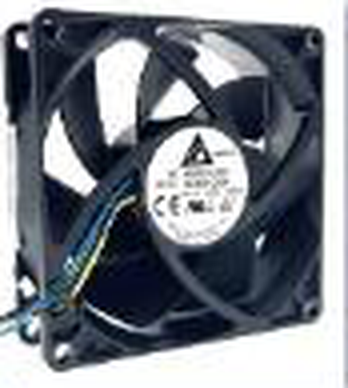
\includegraphics[height=2.6cm]{imagenes/ventilador.png}};

  % título
  \node[anchor=north west, text width=8.6cm, align=left, font=\Large\bfseries]
    at ([xshift=0.9cm,yshift=-0.75cm]current page.north west)
    {Sistema IoT de mantenimiento predictivo para máquinas rotativas mediante monitoreo multimodal y detección de anomalías};

  % datos
  \node[anchor=north west, text width=8.6cm, font=\footnotesize, align=left]
    at ([xshift=0.9cm,yshift=-3.55cm]current page.north west) {%
    \etiq{CURSO}{Internet de las Cosas (CS5055)}
    \etiq{DOCENTE}{Gabriel Andrés Arias Obregón}
    {\color{verde1}\textbf{INTEGRANTES:}}\\[0.05cm]
    \textbf{Josep Ratzinger Castro Ferrer · Jean Paul Cuzcano Ponce}\\
    \textbf{Rodrigo Félix Meza Gavilán · Marcelino Maita Vargas}\\[0.12cm]
    \etiq{CICLO}{2026-2 · Grupo 7}};

  % logo
  \node[anchor=south west] at ([xshift=0.6cm,yshift=0.4cm]current page.south west)
    {
\includegraphics[height=1.4cm]{imagenes/logo_utec.png}};
\end{tikzpicture}
\end{frame}
}

% ================= CONTENIDO =================
\begin{frame}{Contenido}
  \begin{columns}[T]
    \column{0.62\textwidth}
    \tableofcontents
    \column{0.34\textwidth}
    \vspace{0.3cm}
    \begin{block}{Caso de estudio}
      \footnotesize
      Ventilador \textit{brushless} Delta de 12~V vigilado con
      \dato{vibración}, \dato{corriente} y \dato{temperatura}, con inferencia en
      \dato{AWS} y parada por \dato{relé}.
    \end{block}
  \end{columns}
\end{frame}

% =====================================================================
\section{Problemática y contexto}

\begin{frame}{Contexto: las máquinas avisan antes de fallar}
  \begin{columns}[c]
    \column{0.56\textwidth}
    \begin{itemize}\small
      \item Ventiladores, bombas, compresores y motores sostienen la
            \textbf{ventilación, el bombeo y la manufactura}.
      \item Rara vez se detienen sin dar señales previas:
      \begin{itemize}\footnotesize
        \item desbalance u holgura $\rightarrow$ cambia la \dato{vibración};
        \item fricción $\rightarrow$ sube el \dato{consumo eléctrico};
        \item trabajo forzado $\rightarrow$ se acumula \dato{calor}.
      \end{itemize}
      \item Observadas de forma continua, la intervención se puede
            \textbf{planificar antes de la parada}.
      \item El \textbf{IoT abarata esa observación}: medir, enviar a la nube y recibir una orden
            de vuelta.
    \end{itemize}
    \column{0.40\textwidth}
    \centering
    \begin{tikzpicture}
      \node (fan) {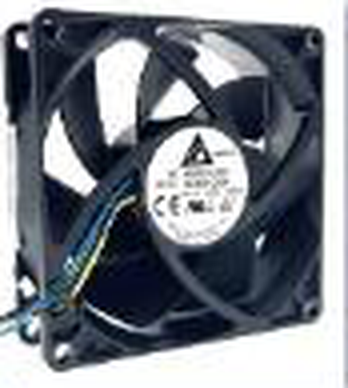
\includegraphics[height=2.9cm]{imagenes/ventilador.png}};
      \node[fuerte, text width=1.75cm, anchor=east] (v) at ([xshift=-0.15cm,yshift=0.9cm]fan.west) {\textbf{Vibración}\\MPU6050};
      \node[fuerte, text width=1.75cm, anchor=east] (c) at ([xshift=-0.15cm,yshift=-0.9cm]fan.west) {\textbf{Corriente}\\ACS712};
      \node[fuerte, text width=1.95cm, anchor=north] (t) at ([yshift=-0.1cm]fan.south) {\textbf{Temperatura}\\DS18B20};
      \draw[flecha] (fan.west) ++(0,0.5) -- (v.east);
      \draw[flecha] (fan.west) ++(0,-0.5) -- (c.east);
      \draw[flecha] (fan.south) -- (t.north);
    \end{tikzpicture}
  \end{columns}
\end{frame}

\begin{frame}{Problemática}
  \small
  En equipos pequeños, las fallas mecánicas (desbalance, holgura, fricción,
  sobrecalentamiento) evolucionan de forma progresiva, pero se detectan
  \textbf{cuando la máquina ya se detuvo}.
  \vspace{0.05cm}

  \renewcommand{\arraystretch}{1.08}
  \footnotesize
  \begin{tabularx}{\textwidth}{@{}>{\bfseries\color{verdeosc}}p{3.7cm}X@{}}
    \toprule
    \color{black}Práctica habitual & \textbf{Limitación} \\
    \midrule
    Inspección esporádica & Solo es una fotografía del instante; los cambios entre visitas pasan
    desapercibidos. \\
    Una sola variable & La corriente varía con la carga, la vibración depende de la fijación y la
    temperatura reacciona tarde. \\
    Alerta sin respuesta & Si nadie actúa a tiempo, detectar el problema no protege al equipo. \\
    \bottomrule
  \end{tabularx}
  \vspace{0.05cm}

  \begin{alertblock}{Pregunta que guía el proyecto}
    \scriptsize
    ¿Puede un sistema IoT de bajo costo reconocer desviaciones del funcionamiento normal de un
    ventilador de 12~V a partir de su vibración, corriente y temperatura, y ordenar su parada
    cuando la desviación persiste?
  \end{alertblock}
  \vspace{0.35cm}
\end{frame}

% =====================================================================
\section{Objetivos}

\begin{frame}{Objetivos}
  \begin{block}{Objetivo general}
    \small
    Diseñar e implementar un prototipo IoT de bajo costo que detecte anomalías en una máquina
    rotativa a partir de la adquisición conjunta de vibración, corriente y temperatura, con
    comunicación inalámbrica, inferencia en la nube y parada controlada mediante relé.
  \end{block}
  \vspace{0.1cm}
  {\small\bfseries\color{verdeosc} Objetivos específicos}
  \vspace{0.05cm}
  \begin{columns}[T]
    \column{0.49\textwidth}
    \begin{enumerate}\footnotesize
      \item Integrar MPU6050, ACS712 y DS18B20 con un ESP32 y caracterizar sus lecturas.
      \item Construir un conjunto de datos de referencia del ventilador.
      \item Entrenar, calibrar y seleccionar un detector de anomalías no supervisado.
    \end{enumerate}
    \column{0.49\textwidth}
    \begin{enumerate}\footnotesize
      \setcounter{enumi}{3}
      \item Implementar la cadena ESP32--IoT Core--Lambda--DynamoDB y el canal de retorno de la
            orden de parada.
      \item Validar el circuito y el firmware en un simulador web.
      \item Encapsular el prototipo separando sensado, control y potencia.
    \end{enumerate}
  \end{columns}
\end{frame}

% =====================================================================
\section{Justificación}

\begin{frame}{Justificación de la solución propuesta}
  \begin{columns}[T]
    \column{0.49\textwidth}
    \begin{block}{1 · Tres variables complementarias}
      \footnotesize Una sola señal es ambigua; combinar vibración, corriente y temperatura reduce
      la ambigüedad.
    \end{block}
    \begin{block}{2 · Detección no supervisada}
      \footnotesize No hay un catálogo de fallas etiquetadas: Isolation Forest aprende solo de la
      operación normal.
    \end{block}
    \column{0.49\textwidth}
    \begin{block}{3 · Lazo cerrado}
      \footnotesize Detectar sin actuar no protege: tras \textbf{3 anomalías seguidas} se puede
      ordenar la apertura del relé.
    \end{block}
    \begin{block}{4 · Nube sin servidores}
      \footnotesize Sin laptop encendida, autenticación por certificado, registro persistente y
      costo solo cuando llega un mensaje.
    \end{block}
  \end{columns}
  \vspace{0.15cm}
  \begin{alertblock}{Cambios respecto del perfil (P1)}
    \footnotesize
    \textbf{RCF $\rightarrow$ Isolation Forest:} RCF en AWS requiere un punto de inferencia de
    SageMaker con costo por hora; Isolation Forest se entrena en segundos y cabe en una imagen de
    Lambda.\quad
    \textbf{Laptop $\rightarrow$ AWS:} elimina la dependencia de una laptop en la misma red.
  \end{alertblock}
\end{frame}

% =====================================================================
\section{Estado del arte}

\begin{frame}{Estado del arte}
  \scriptsize
  \renewcommand{\arraystretch}{1.18}
  \begin{tabularx}{\textwidth}{@{}>{\raggedright\arraybackslash\bfseries\color{verdeosc}}p{2.2cm}>{\raggedright\arraybackslash}p{2.75cm}>{\raggedright\arraybackslash}X>{\raggedright\arraybackslash}X@{}}
    \toprule
    \color{black}Línea & \textbf{Trabajos} & \textbf{Hallazgo} & \textbf{Decisión en el prototipo} \\
    \midrule
    Máquinas rotativas & Tiboni 2022; Niu 2023; Lei 2020 &
    El diagnóstico depende de la adquisición; la corriente es complementaria; casi todo estudio
    usa fallas etiquetadas. &
    MPU6050 fijado rígido; corriente junto a otras variables; enfoque no supervisado. \\
    ML para mantenimiento predictivo & Carvalho 2019; Zhang 2019; Zonta 2020; \c{C}{\i}nar 2020;
    Serradilla 2022 &
    Predominan métodos supervisados; arquitectura en capas; integrar modelo y decisión es un reto;
    el aprendizaje profundo exige muchos datos. &
    Sin clasificadores supervisados; sistema en capas; lazo cerrado; modelo ligero en Lambda. \\
    Detección de anomalías & Pang 2021; Hariri 2021 &
    Usar líneas base clásicas; los cortes paralelos a los ejes generan artefactos. &
    Isolation Forest con escalado robusto previo. \\
    Infraestructura IoT & Compare 2020; Mishra y Kertesz 2020 &
    Continuidad, seguridad y decisión local; MQTT es ligero y con QoS. &
    Certificados X.509; MQTT sobre TLS; relé con control local. \\
    \bottomrule
  \end{tabularx}
\end{frame}

\begin{frame}{Brecha y figura basada en el estado del arte}
  \begin{alertblock}{La brecha no es algorítmica, sino de integración}
    \footnotesize
    Demostrar la cadena completa ---sensado, inferencia y actuación--- con componentes de bajo
    costo y servicios gestionados en la nube.
  \end{alertblock}
  \vspace{0.25cm}
  \centering
  \resizebox{\textwidth}{!}{%
  \begin{tikzpicture}
    \node[caja, fill=white, text width=2.45cm] (l1) at (0,0)    {\textbf{Adquisición}\\señales físicas del activo};
    \node[caja, fill=white, text width=2.45cm] (l2) at (2.95,0) {\textbf{Preprocesamiento}\\en el borde y transmisión};
    \node[caja, fill=white, text width=2.45cm] (l3) at (5.9,0)  {\textbf{Modelado}\\puntaje de anomalía};
    \node[caja, fill=white, text width=2.45cm] (l4) at (8.85,0) {\textbf{Decisión}\\persistencia y criterio};
    \node[caja, fill=white, text width=2.45cm] (l5) at (11.8,0) {\textbf{Actuación}\\protección del equipo};
    \node[fuerte, text width=2.45cm] (p1) at (0,-1.75)    {MPU6050 · ACS712 · DS18B20\\sobre el ventilador};
    \node[fuerte, text width=2.45cm] (p2) at (2.95,-1.75) {ESP32: lectura completa,\\JSON y MQTT/TLS};
    \node[fuerte, text width=2.45cm] (p3) at (5.9,-1.75)  {Lambda: escalado robusto\\+ Isolation Forest};
    \node[fuerte, text width=2.45cm] (p4) at (8.85,-1.75) {DynamoDB: contador de\\3 anomalías seguidas};
    \node[fuerte, text width=2.45cm] (p5) at (11.8,-1.75) {Orden OFF $\rightarrow$ relé\\corta 12~V};
    \foreach \a/\b in {1/2,2/3,3/4,4/5} {
      \draw[flecha] (l\a) -- (l\b);
      \draw[flecha] (p\a) -- (p\b);
    }
    \foreach \i in {1,...,5} \draw[dotted, verdeosc, thick] (l\i) -- (p\i);
    \node[font=\scriptsize\itshape, anchor=east] at ($(l1.west)+(-0.15,0)$) {Literatura};
    \node[font=\scriptsize\itshape, anchor=east] at ($(p1.west)+(-0.15,0)$) {Prototipo};
  \end{tikzpicture}}
  \vspace{0.1cm}

  {\tiny\color{gray} Capas del mantenimiento predictivo dirigido por datos (Zhang 2019; Compare 2020)
  y su implementación en el prototipo.}
\end{frame}

% =====================================================================
\section{Fundamentos teóricos y tecnologías utilizadas}

\begin{frame}{Fundamentos teóricos y tecnologías utilizadas}{Conceptos clave}
  \begin{columns}[T]
    \column{0.32\textwidth}
    \begin{block}{Mantenimiento basado en condición}
      \scriptsize
      Se interviene según el \textbf{estado medido} de la máquina, no por calendario ni después de
      la falla. Tres señales describen ese estado:\\[4pt]
      \centering
      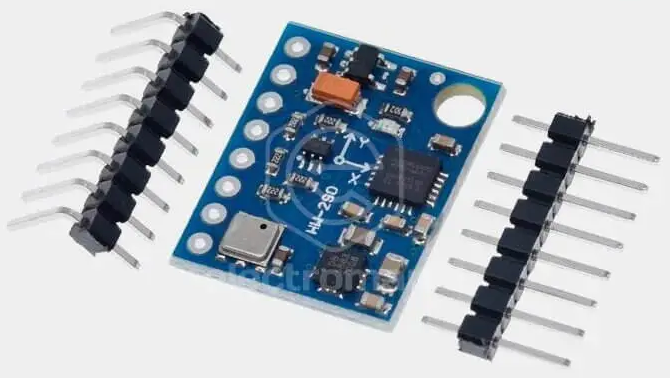
\includegraphics[height=0.75cm]{imagenes/mpu6050.png}\hfill
      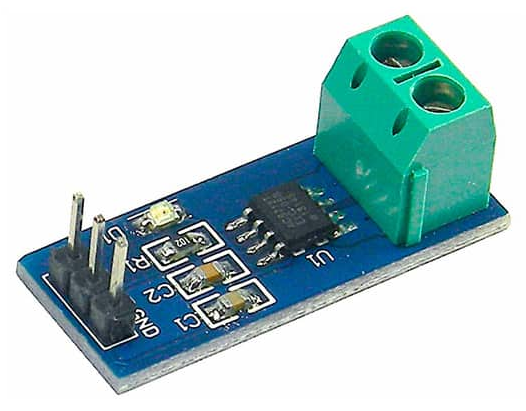
\includegraphics[height=0.75cm]{imagenes/acs712.png}\hfill
      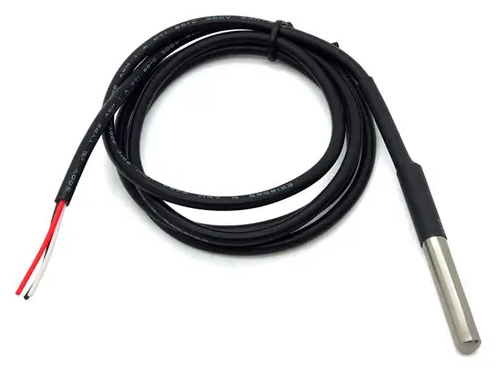
\includegraphics[height=0.75cm]{imagenes/ds18b20.png}\\[2pt]
      \raggedright
      \dato{Vibración} (MPU6050), \dato{corriente} (ACS712, efecto Hall) y
      \dato{temperatura} (DS18B20, 1-Wire).
    \end{block}
    \column{0.32\textwidth}
    \begin{block}{Isolation Forest}
      \scriptsize
      Lo anómalo es \textbf{escaso y distinto}: se aísla con menos cortes aleatorios que lo normal.
      Aprende \textbf{solo de la operación normal}.\\[3pt]
      \centering
      \begin{tikzpicture}[scale=0.42]
        \fill[white] (0,0) rectangle (4.6,3.4);
        \draw[verde1, thick] (0,0) rectangle (4.6,3.4);
        \draw[rojo, very thick] (1.3,0) -- (1.3,3.4);
        \draw[rojo, very thick] (0,2.2) -- (1.3,2.2);
        \draw[verdeosc, thin] (3.6,0) -- (3.6,3.4);
        \draw[verdeosc, thin] (1.3,1.1) -- (3.6,1.1);
        \draw[verdeosc, thin] (2.4,1.1) -- (2.4,3.4);
        \draw[verdeosc, thin] (2.4,2.3) -- (3.6,2.3);
        \draw[verdeosc, thin] (2.9,1.1) -- (2.9,2.3);
        \draw[verdeosc, thin] (2.4,1.7) -- (2.9,1.7);
        \foreach \x/\y in {2.5/1.5,2.7/1.9,2.6/1.3,2.8/1.6,3.0/1.8,3.1/1.4,2.55/2.0,
                           3.2/2.0,2.3/1.6,2.95/1.25,3.3/1.65,2.7/2.2}
          \fill[verdeosc] (\x,\y) circle (0.08);
        \fill[rojo] (0.6,2.8) circle (0.13);
      \end{tikzpicture}\\[2pt]
      \raggedright
      En el modelo final: lectura típica \dato{12.7 cortes}, anómala \dato{3.4}.
    \end{block}
    \column{0.32\textwidth}
    \begin{block}{MQTT sobre AWS IoT Core}
      \scriptsize
      Protocolo ligero de \textbf{publicación/suscripción} por tópicos; un \emph{broker} reparte
      los mensajes.\\[4pt]
      \centering
      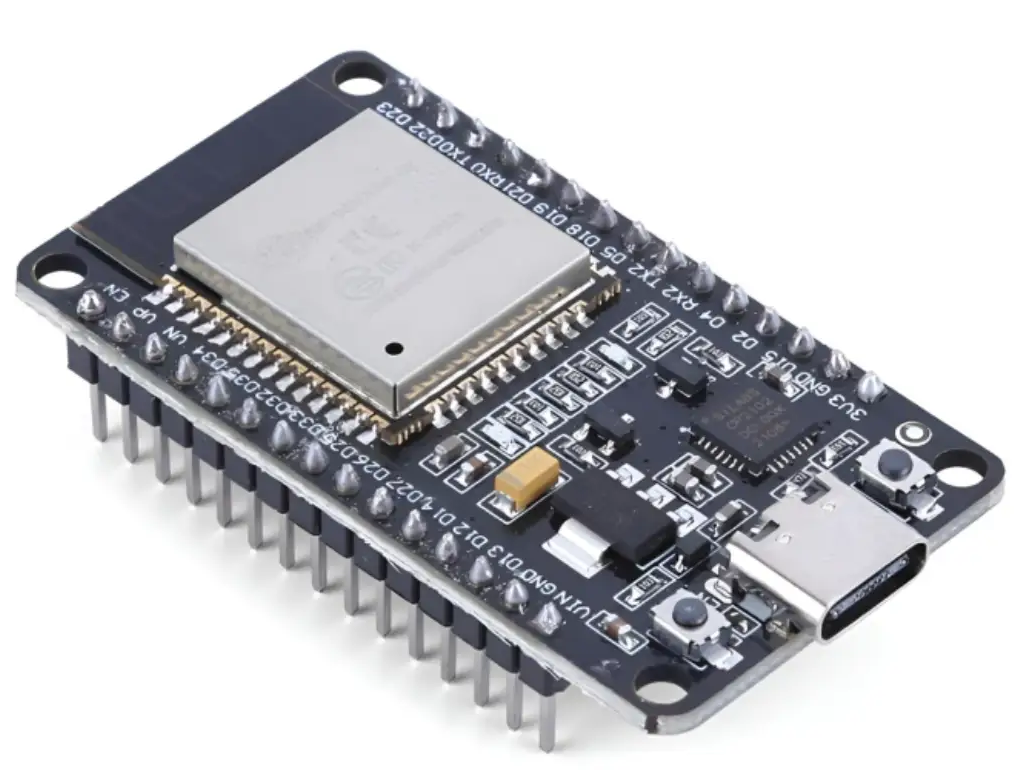
\includegraphics[height=0.9cm]{imagenes/esp32.png}\\[2pt]
      \raggedright
      El ESP32 publica lecturas en \code{esp32/pub} y recibe la orden ON/OFF en \code{esp32/sub},
      autenticado con \textbf{TLS mutuo} y certificados X.509.
    \end{block}
  \end{columns}
\end{frame}

\begin{frame}{Fundamentos teóricos y tecnologías utilizadas}{Tecnologías utilizadas}
  \footnotesize
  \renewcommand{\arraystretch}{1.25}
  \begin{tabularx}{\textwidth}{@{}>{\raggedright\arraybackslash\bfseries\color{verdeosc}}p{2.9cm}>{\raggedright\arraybackslash}p{4.6cm}>{\raggedright\arraybackslash}X@{}}
    \toprule
    \color{black}Parte del proyecto & \textbf{Tecnologías} & \textbf{Para qué se usan} \\
    \midrule
    Conexiones y armado & ESP32 DevKit V1, MPU6050, ACS712, DS18B20, módulo de relé, fuente
    de 12~V & Adquirir las tres señales y cortar la alimentación del ventilador. \\
    Simulación & TypeScript, Three.js, React Three Fiber (navegador) & Réplica 3D del circuito y
    del firmware para probar fallas sin arriesgar componentes. \\
    Modelo de ML & Python, pandas, scikit-learn (Isolation Forest), joblib & Entrenar y
    seleccionar el detector; exportarlo como \code{best\_model.joblib}. \\
    Conexión con AWS & MQTT/TLS, AWS IoT Core, AWS Lambda (contenedor en ECR), DynamoDB, AWS SAM &
    Recibir lecturas, ejecutar la inferencia, guardar el historial y devolver la orden de parada. \\
    \bottomrule
  \end{tabularx}
\end{frame}

% =====================================================================
\section{Desarrollo conceptual de la solución}

\begin{frame}{Desarrollo conceptual de la solución}{Arquitectura del sistema}
  \centering
  \resizebox{!}{4.9cm}{%
  \begin{tikzpicture}
    % bandas
    \begin{scope}[on background layer]
      \fill[banda] (-0.15,-2.55) rectangle (2.15,1.35);
      \fill[banda] (2.4,-2.55) rectangle (4.6,1.35);
      \fill[banda] (4.85,-2.75) rectangle (9.15,1.35);
      \fill[banda] (9.4,-1.05) rectangle (11.65,1.35);
    \end{scope}
    \node[titbanda] at (1.0,1.05) {Percepción};
    \node[titbanda] at (3.5,1.05) {Borde};
    \node[titbanda] at (7.0,1.05) {Nube AWS};
    \node[titbanda] at (10.52,1.05) {Visualización};
    % nodos
    \node[caja, text width=1.9cm, minimum height=1.25cm] (fan) at (1.0,0) {\textbf{Ventilador 12~V}\\MPU6050\\ACS712 · DS18B20};
    \node[oscura, text width=1.85cm, minimum height=1.25cm] (esp) at (3.5,0) {\textbf{ESP32}\\lectura + JSON\\MQTT/TLS};
    \node[oscura, text width=3.6cm, minimum height=1.25cm] (aws) at (7.0,0) {\textbf{Inferencia y registro}\\Isolation Forest por lectura\\contador de anomalías};
    \node[caja, text width=1.85cm, minimum height=1.25cm] (web) at (10.52,0) {\textbf{API HTTP}\\monitor web\\gemelo 3D};
    \node[caja, fill=rojo!12, draw=rojo, text width=1.85cm] (rele) at (3.5,-1.85) {\textbf{Relé}\\activo en bajo};
    \node[caja, fill=white, draw=gray, text width=3.4cm] (lap) at (7.0,-2.0) {\textbf{Entrenamiento} (fuera de línea)\\VentiSet.csv $\rightarrow$ \code{.joblib}};
    \node[caja, fill=white, draw=gray, dashed, text width=4.4cm] (sim) at (2.25,-3.5) {\textbf{Simulador 3D}: réplica virtual de\\sensores, ESP32 y relé antes del montaje};
    % datos
    \draw[flecha] ([yshift=0.25cm]fan.east) -- node[etq, above=1pt]{3 señales} ([yshift=0.25cm]esp.west);
    \draw[flecha] ([yshift=0.25cm]esp.east) -- node[etq, above=1pt]{\code{esp32/pub}} ([yshift=0.25cm]aws.west);
    \draw[flecha] ([yshift=0.25cm]aws.east) -- node[etq, above=1pt]{consulta} ([yshift=0.25cm]web.west);
    % retorno
    \draw[retorno] ([yshift=-0.3cm]aws.west) -- node[etq, below=1pt]{OFF tras\\3 anomalías} ([yshift=-0.3cm]esp.east);
    \draw[retorno] (esp.south) -- node[etq, right=1pt]{GPIO26} (rele.north);
    \draw[retorno] (rele.west) -| node[etq, pos=0.3, below=1pt]{corta 12~V} (fan.south);
    \draw[punteada] (lap.north) -- node[etq, right=1pt]{modelo} (aws.south);
    \draw[punteada] (sim.north) -- ++(0,0.4);
  \end{tikzpicture}}
  \vspace{0.15cm}

  {\scriptsize Flechas verdes: datos. Rojas: cadena de actuación. Punteadas: trabajo fuera de
  línea (entrenamiento y simulación).}
\end{frame}


% ---------------- Conexiones ----------------
\begin{frame}{Desarrollo conceptual de la solución}{Conexiones e interconexión de componentes}
  \begin{columns}[c]
    \column{0.47\textwidth}
    \scriptsize
    \renewcommand{\arraystretch}{1.25}
    \begin{tabularx}{\linewidth}{@{}>{\bfseries\color{verdeosc}}l c X@{}}
      \toprule
      \color{black}Componente & \textbf{GPIO} & \textbf{Conexión} \\
      \midrule
      MPU6050 & 21, 22 & I$^2$C (SDA, SCL), 3.3~V \\
      DS18B20 & 4 & 1-Wire, \textit{pull-up} 5~k$\Omega$ (2 de 10~k$\Omega$ en paralelo) \\
      ACS712 & 34 & ADC1 por divisor (2 de 10~k$\Omega$ en serie) \\
      Relé & 26 & IN2, activo en nivel bajo \\
      \bottomrule
    \end{tabularx}
    \vspace{0.25cm}

    {\footnotesize\bfseries\color{verdeosc} Rama de potencia (12~V)}\\[3pt]
    \resizebox{\linewidth}{!}{%
    \begin{tikzpicture}[node distance=0.3cm]
      \node[caja, minimum height=0.5cm, font=\tiny] (r1) {Fuente $+$};
      \node[caja, minimum height=0.5cm, font=\tiny, right=of r1] (r2) {COM2};
      \node[caja, minimum height=0.5cm, font=\tiny, right=of r2] (r3) {NO2};
      \node[fuerte, minimum height=0.5cm, font=\tiny, right=of r3] (r4) {ACS712};
      \node[caja, minimum height=0.5cm, font=\tiny, right=of r4] (r5) {Ventilador};
      \node[caja, minimum height=0.5cm, font=\tiny, right=of r5] (r6) {Fuente $-$};
      \draw[flecha] (r1) -- (r2); \draw[flecha] (r2) -- (r3); \draw[flecha] (r3) -- (r4);
      \draw[flecha] (r4) -- (r5); \draw[flecha] (r5) -- (r6);
    \end{tikzpicture}}\\[3pt]
    \scriptsize Al cerrar COM2--NO2, la corriente del ventilador atraviesa el ACS712. La rama de
    potencia queda separada de la alimentación USB del ESP32.
    \column{0.51\textwidth}
    \centering
    \imagen{imagenes/prototipo_armado/diagrama-interconexiones.png}{\linewidth}{4.7cm}
  \end{columns}
\end{frame}

\begin{frame}{Desarrollo conceptual de la solución}{Armado del prototipo}
  \begin{columns}[T]
    \column{0.32\textwidth}
    \centering
    \imagen{imagenes/prototipo_armado/montaje-abierto.jpg}{\linewidth}{3.2cm}\\[3pt]
    \scriptsize Montaje abierto: ESP32 por USB, protoboard y módulos en la rama del ventilador.
    \column{0.32\textwidth}
    \centering
    \imagen{imagenes/prototipo_armado/rele-cableado.jpg}{\linewidth}{3.2cm}\\[3pt]
    \scriptsize Detalle del relé y del ACS712 junto a la protoboard.
    \column{0.32\textwidth}
    \centering
    \imagen{imagenes/prototipo_armado/monitor-serie.jpg}{\linewidth}{3.2cm}\\[3pt]
    \scriptsize Monitor serie: 27.25~$^\circ$C, aceleración en 3 ejes y ${\sim}1361$~mV en el
    ACS712.
  \end{columns}
  \vspace{0.25cm}
  \begin{block}{Firmware de prueba}
    \footnotesize Comandos serie \code{L}/\code{H} para conmutar el relé; lectura de los tres
    sensores en cada ciclo y promedio de 64 muestras del ADC para el ACS712.
  \end{block}
\end{frame}

% ---------------- Simulación ----------------
\begin{frame}{Desarrollo conceptual de la solución}{Simulación del armado en la web}
  \begin{columns}[T,totalwidth=\textwidth]
    \column{0.45\textwidth}
    \begin{itemize}\scriptsize
      \item \textbf{Simulador 3D propio} en el navegador, sin instalación.
      \item Reproduce \textbf{agujero por agujero} el cableado real.
      \item \textbf{Modelo físico a 2~kHz}: desbalance, holgura, fricción y calentamiento.
      \item Sensores con sus límites reales (16~bits, 750~ms, 185~mV/A).
      \item Permite \textbf{inyectar fallas} y seguir las variables en vivo.
    \end{itemize}
    \vspace{0.1cm}
    \begin{alertblock}{Resultado}
      \scriptsize Con falla, el relé abrió \dato{5~ms} después del estado crítico; sin Wi-Fi, el
      límite local de 60~$^\circ$C detuvo el ventilador.
    \end{alertblock}
    \column{0.52\textwidth}
    \centering
    \imagen{imagenes/simulador/SIM_01.png}{\linewidth}{2.3cm}\\[3pt]
    \imagen{imagenes/simulador/SIM_03.png}{\linewidth}{2.3cm}\\[1pt]
    \parbox{\linewidth}{\centering\tiny\color{gray} Vista general y escenario de
    sobrecalentamiento.}
  \end{columns}
  \vspace{0.4cm}
\end{frame}

% ---------------- Modelo ML ----------------
\begin{frame}{Desarrollo conceptual de la solución}{Modelo de detección de anomalías}
  \centering
  \resizebox{\textwidth}{!}{%
  \begin{tikzpicture}
    \node[caja, text width=2.05cm] (a) at (0,0) {\textbf{VentiSet.csv}\\4\,261 registros\\69~min};
    \node[caja, text width=2.05cm] (b) at (2.6,0) {\textbf{Selección}\\3\,927 ENCENDIDO\\5 variables};
    \node[fuerte, text width=2.25cm] (c) at (5.3,0) {\textbf{Partición cronológica}\\70/15/15\\2\,748 · 589 · 590};
    \node[fuerte, text width=2.35cm] (d) at (8.1,0) {\textbf{Pipeline}\\mediana $\rightarrow$\\RobustScaler $\rightarrow$ IF};
    \node[fuerte, text width=2.25cm] (e) at (10.9,0) {\textbf{12 candidatos}\\$U=\mathrm{TDS}-2\,\mathrm{FPR}$\\$\mathrm{FPR}\leq5\,\%$};
    \node[oscura, text width=2.25cm] (f) at (13.6,0) {\textbf{Modelo \#12}\\400 árboles, $\psi=256$\\umbral 0.528};
    \foreach \x/\y in {a/b,b/c,c/d,d/e,e/f} \draw[flecha] (\x) -- (\y);
  \end{tikzpicture}}
  \vspace{0.15cm}

  \begin{columns}[c]
    \column{0.36\textwidth}
    \centering
    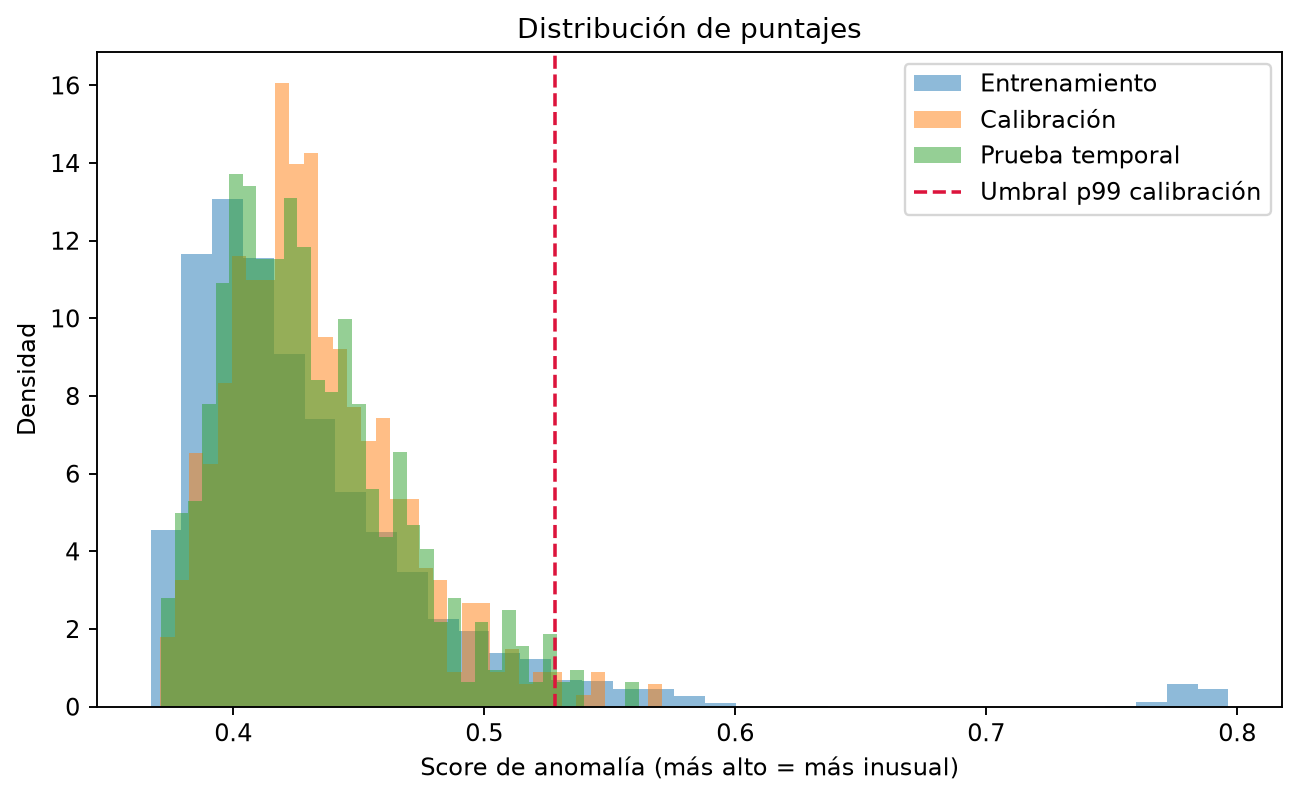
\includegraphics[width=\linewidth,height=2.8cm,keepaspectratio]{imagenes/resultados/03_scores.png}\\
    {\tiny\color{gray} Puntaje por bloque frente al umbral p99.}
    \column{0.36\textwidth}
    \centering
    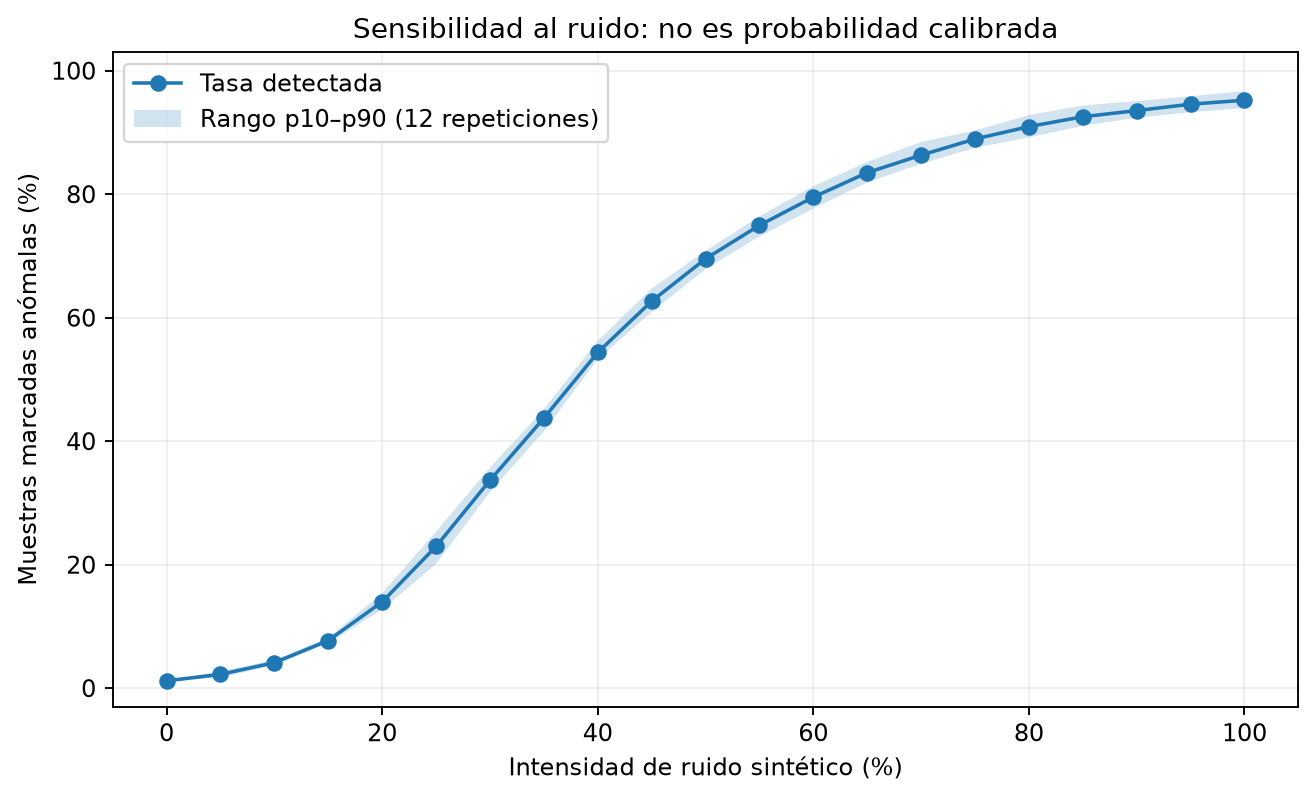
\includegraphics[width=\linewidth,height=2.8cm,keepaspectratio]{imagenes/resultados/06_ruido_tasa_anomalias.png}\\
    {\tiny\color{gray} Lecturas marcadas según la perturbación.}
    \column{0.25\textwidth}
    \scriptsize
    \dato{FPR 1.02\,\%}\\ en validación\\[3pt]
    \dato{83.1\,\%} de detección\\ sintética\\[3pt]
    \dato{7 de 590} lecturas de\\ prueba marcadas (1.19\,\%), sin 3 seguidas
  \end{columns}
\end{frame}

% ---------------- AWS ----------------
\begin{frame}{Desarrollo conceptual de la solución}{Conexión con AWS}
  \centering
  \vspace{-0.15cm}
  \begin{tikzpicture}[
      metrica/.style={draw=verdeosc, fill=verde5, rounded corners=3pt, line width=0.7pt,
                      text width=2.05cm, align=center, font=\tiny, inner sep=2.5pt}]
    \node[inner sep=0, anchor=south west] (img) at (0,0)
      {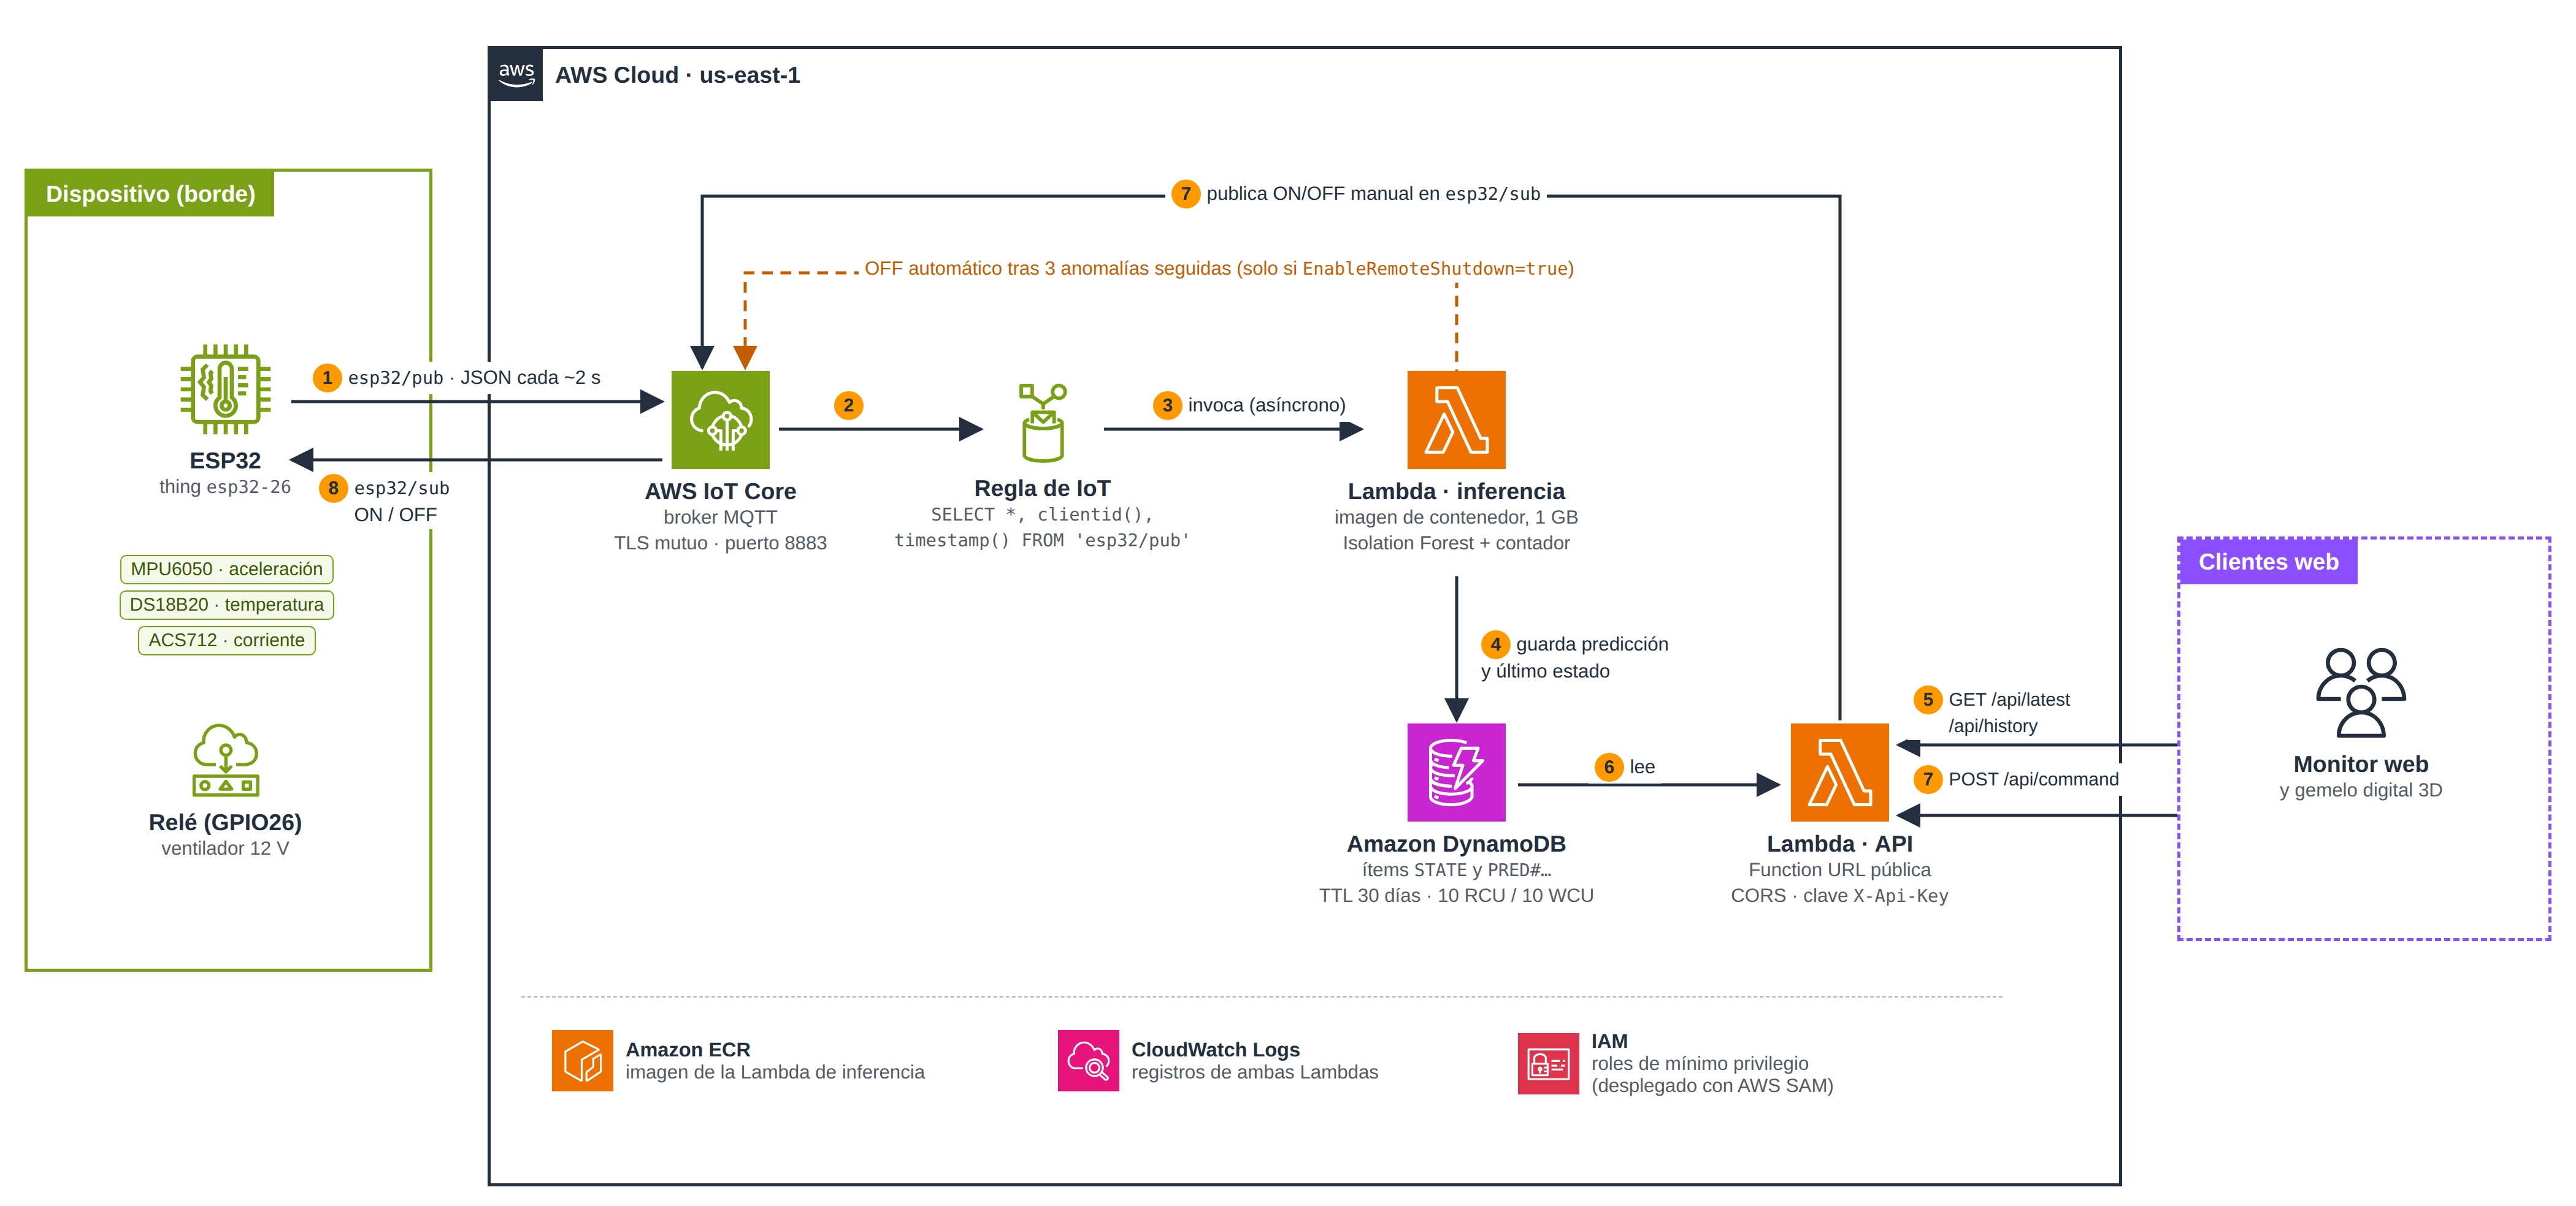
\includegraphics[width=\textwidth,height=6.4cm,keepaspectratio]{aws/arquitectura-aws.png}};
    % coordenadas relativas a la imagen: (0,0) esquina inferior izquierda, (1,1) superior derecha
    \begin{scope}[x={(img.south east)}, y={(img.north west)}]
      % esquina superior derecha (espacio libre sobre "Clientes web")
      \node[metrica] at (0.913,0.80)
        {\textbf{\color{verdeosc}Inferencia en Lambda}\\[1pt]
         {\scriptsize\bfseries ${\sim}84$~ms}\\ por lectura en caliente};
      % esquina inferior derecha (debajo de "Clientes web")
      \node[metrica] at (0.913,0.10)
        {\textbf{\color{verdeosc}Consultas a la API}\\[1pt]
         {\scriptsize\bfseries 10--121~ms}\\ sin clave $\rightarrow$ \code{401}};
      % esquina inferior izquierda (debajo del dispositivo)
      \node[metrica] at (0.093,0.10)
        {\textbf{\color{verdeosc}Orden OFF $\rightarrow$ relé}\\[1pt]
         {\scriptsize\bfseries 3.6--7.2~s}\\ media 5.3~s};
    \end{scope}
  \end{tikzpicture}
\end{frame}

% =====================================================================
\section{Síntesis}

\begin{frame}{Síntesis}
  \begin{columns}[T]
    \column{0.49\textwidth}
    \begin{block}{Lo logrado}
      \footnotesize
      \begin{itemize}
        \item Cadena completa: tres sensores, ESP32, MQTT/TLS, inferencia en AWS y relé de
              parada.
        \item Conjunto de datos real (3\,927 lecturas) y detector Isolation Forest con
              partición cronológica.
        \item Simulador 3D y API para el monitor web y el gemelo digital.
      \end{itemize}
    \end{block}
    \column{0.49\textwidth}
    \begin{alertblock}{Siguientes pasos}
      \footnotesize
      \begin{itemize}
        \item Muestrear el MPU6050 a cientos de hercios y calcular RMS y factor de cresta.
        \item Registrar fallas inducidas y etiquetadas para medir sensibilidad real.
        \item Límites locales de corriente y temperatura en el firmware.
      \end{itemize}
    \end{alertblock}
  \end{columns}
\end{frame}

% ================= CIERRE =================
{
\setbeamertemplate{background}{\begin{tikzpicture}[remember picture,overlay]
  \fill[verde1] (current page.south west) rectangle (current page.north east);
  \fill[verde2] ([xshift=5cm]current page.north) -- (current page.north east) -- (current page.south east) -- ([xshift=1cm]current page.south) -- cycle;
  \fill[verde3] ([xshift=7cm]current page.north) -- (current page.north east) -- (current page.south east) -- ([xshift=4cm]current page.south) -- cycle;
\end{tikzpicture}}
\begin{frame}[plain]
\begin{tikzpicture}[remember picture,overlay,line join=round,line cap=round]
  \begin{scope}[shift={([xshift=-4.2cm,yshift=-2.2cm]current page.center)},scale=0.9]
    % sombra
    \fill[verdeosc,opacity=0.25] (0.9,-0.15) ellipse (2.4 and 0.22);
    \tikzset{piel/.style={fill=verde5,draw=verdeosc,very thick}}
    % cola
    \fill[piel] (-0.2,2.1) .. controls (-1.2,1.9) and (-2.2,1.2) .. (-2.9,0.6)
      .. controls (-2.0,0.9) and (-1.0,1.2) .. (0.0,1.3) -- cycle;
    % piernas (antes del cuerpo, para que su parte de arriba quede tapada)
    \fill[piel] (0.4,1.3) -- (0.35,-0.1) -- (0.95,-0.1) -- (0.95,1.3) -- cycle;
    \fill[piel] (1.15,1.3) -- (1.1,-0.1) -- (1.7,-0.1) -- (1.65,1.3) -- cycle;
    % cuerpo inclinado
    \fill[piel,rotate around={30:(0.8,1.9)}] (0.8,1.9) ellipse (1.35 and 0.85);
    % cuello
    \fill[piel] (1.2,2.3) -- (1.7,3.4) -- (2.5,3.1) -- (1.9,1.9) -- cycle;
    % muslo (dentro del cuerpo, sobre la pierna)
    \fill[piel] (0.75,1.55) circle (0.48);
    % garras de los pies
    \foreach \x in {0.37,0.6,0.83,1.12,1.35,1.58} \fill[white,draw=verdeosc,thin] (\x,-0.1) -- ++(0.06,-0.12) -- ++(0.06,0.12) -- cycle;
    % mandíbula inferior (boca abierta)
    \fill[piel,rounded corners=6pt] (1.9,3.2) -- (3.5,3.05) -- (3.35,2.7) -- (2.0,2.7) -- cycle;
    \fill[pink!60,rounded corners=4pt] (2.3,3.15) -- (3.35,3.06) -- (3.2,2.9) -- (2.4,2.92) -- cycle;
    % dientes inferiores
    \foreach \x in {2.55,2.85,3.15} \fill[white,draw=verdeosc,thin] (\x,3.07) -- ++(0.07,0.15) -- ++(0.07,-0.15) -- cycle;
    % cráneo
    \fill[piel,rounded corners=10pt] (1.6,3.2) -- (1.75,4.1) -- (3.75,4.0) -- (3.9,3.3) -- cycle;
    % dientes superiores
    \foreach \x in {2.4,2.7,3.0,3.3,3.6} \fill[white,draw=verdeosc,thin] (\x,3.27) -- ++(0.07,-0.17) -- ++(0.07,0.17) -- cycle;
    % ojo y fosa nasal
    \fill[white,draw=verdeosc,thick] (2.45,3.72) circle (0.2);
    \fill[black] (2.52,3.73) circle (0.1); \fill[white] (2.55,3.77) circle (0.03);
    \fill[verdeosc] (3.6,3.82) ellipse (0.07 and 0.04);
    % bracitos
    \draw[verdeosc,line width=4pt] (1.95,2.35) -- (2.35,2.15) -- (2.45,2.3);
    \draw[verde5,line width=2pt] (1.95,2.35) -- (2.35,2.15) -- (2.45,2.3);
    % manchas
    \fill[verde3] (0.4,2.1) circle (0.2); \fill[verde3] (1.0,2.4) circle (0.14);
    \fill[verde3] (0.9,1.7) circle (0.17); \fill[verde3] (2.6,3.55) circle (0.08);
    % púas en la espalda
    \foreach \x/\y/\r in {-0.6/1.85/20,0.0/2.25/25,0.55/2.6/30,1.05/2.95/40,1.45/3.45/55}
      \fill[verdeosc,rotate around={\r:(\x,\y)}] (\x,\y) -- ++(0.14,0.26) -- ++(0.14,-0.26) -- cycle;
    % globo de diálogo: primero la punta, luego el globo encima
    \fill[white,draw=verdeosc,very thick] (6.4,4.6) -- (6.4,4.0) -- (4.0,3.4) -- cycle;
    \node[fill=white,draw=verdeosc,very thick,rounded corners=12pt,inner sep=10pt,
          font=\Huge\bfseries,text=verdeosc] at (8.2,4.4) {¡Gracias!};
  \end{scope}
\end{tikzpicture}
\end{frame}
}

\end{document}
